% Shared LaTeX preamble for 权衡司南 entries.
% Every entry pulls this in with % Shared LaTeX preamble for 权衡司南 entries.
% Every entry pulls this in with % Shared LaTeX preamble for 权衡司南 entries.
% Every entry pulls this in with \input{../../templates/preamble}.
% Do not copy this file into an entry. One file, one source of truth.
%
% Engine note: the content is Mandarin, so entries are built with XeLaTeX
% (see the Makefile LATEX variable and the CI workflow). pdfLaTeX cannot set
% CJK body text. The iftex guard below keeps a pdfLaTeX run from hard-failing
% on the fontspec/ctex packages, but only XeLaTeX or LuaLaTeX produces correct
% Mandarin output.

\usepackage{iftex}

\usepackage{xcolor}
\definecolor{Primary}{HTML}{5C1D74}   % deep purple
\definecolor{Secondary}{HTML}{E5C300} % yellow
\definecolor{Tertiary}{HTML}{1D7466}  % teal

\ifPDFTeX
  \usepackage[T1]{fontenc}
  \usepackage[utf8]{inputenc}
\else
  % XeLaTeX / LuaLaTeX: Unicode engine with CJK support for Mandarin.
  \usepackage{fontspec}
  \usepackage{ctex}
\fi

\usepackage{amsmath}
\usepackage{amssymb}
\usepackage{amsthm}

\usepackage{graphicx}
\graphicspath{{figures/}}
% SVG figures are included via the svg package (needs inkscape + -shell-escape).
% GIF figures never enter the PDF; the HTML version references the GIF instead.
\usepackage{svg}

\usepackage[colorlinks=true, linkcolor=Primary, urlcolor=Tertiary,
            citecolor=Tertiary]{hyperref}
.
% Do not copy this file into an entry. One file, one source of truth.
%
% Engine note: the content is Mandarin, so entries are built with XeLaTeX
% (see the Makefile LATEX variable and the CI workflow). pdfLaTeX cannot set
% CJK body text. The iftex guard below keeps a pdfLaTeX run from hard-failing
% on the fontspec/ctex packages, but only XeLaTeX or LuaLaTeX produces correct
% Mandarin output.

\usepackage{iftex}

\usepackage{xcolor}
\definecolor{Primary}{HTML}{5C1D74}   % deep purple
\definecolor{Secondary}{HTML}{E5C300} % yellow
\definecolor{Tertiary}{HTML}{1D7466}  % teal

\ifPDFTeX
  \usepackage[T1]{fontenc}
  \usepackage[utf8]{inputenc}
\else
  % XeLaTeX / LuaLaTeX: Unicode engine with CJK support for Mandarin.
  \usepackage{fontspec}
  \usepackage{ctex}
\fi

\usepackage{amsmath}
\usepackage{amssymb}
\usepackage{amsthm}

\usepackage{graphicx}
\graphicspath{{figures/}}
% SVG figures are included via the svg package (needs inkscape + -shell-escape).
% GIF figures never enter the PDF; the HTML version references the GIF instead.
\usepackage{svg}

\usepackage[colorlinks=true, linkcolor=Primary, urlcolor=Tertiary,
            citecolor=Tertiary]{hyperref}
.
% Do not copy this file into an entry. One file, one source of truth.
%
% Engine note: the content is Mandarin, so entries are built with XeLaTeX
% (see the Makefile LATEX variable and the CI workflow). pdfLaTeX cannot set
% CJK body text. The iftex guard below keeps a pdfLaTeX run from hard-failing
% on the fontspec/ctex packages, but only XeLaTeX or LuaLaTeX produces correct
% Mandarin output.

\usepackage{iftex}

\usepackage{xcolor}
\definecolor{Primary}{HTML}{5C1D74}   % deep purple
\definecolor{Secondary}{HTML}{E5C300} % yellow
\definecolor{Tertiary}{HTML}{1D7466}  % teal

\ifPDFTeX
  \usepackage[T1]{fontenc}
  \usepackage[utf8]{inputenc}
\else
  % XeLaTeX / LuaLaTeX: Unicode engine with CJK support for Mandarin.
  \usepackage{fontspec}
  \usepackage{ctex}
\fi

\usepackage{amsmath}
\usepackage{amssymb}
\usepackage{amsthm}

\usepackage{graphicx}
\graphicspath{{figures/}}
% SVG figures are included via the svg package (needs inkscape + -shell-escape).
% GIF figures never enter the PDF; the HTML version references the GIF instead.
\usepackage{svg}

\usepackage[colorlinks=true, linkcolor=Primary, urlcolor=Tertiary,
            citecolor=Tertiary]{hyperref}


\title{RoPE 是怎么被逼出来的}
\date{2026-09-01}

\begin{document}

旋转位置编码（RoPE）把每个 query 和 key 按它所在的绝对位置转过一个角度，转过之后，两个向量的点积就只依赖于它们之间的相对距离。这一句话生成了其余的全部。下面不是对方法的复述，而是把它一步步逼出来：每一步都由上一步的缺口决定，没有一处是选来的。假设读者熟悉点积、矩阵乘法和注意力的形状，不假设读者见过任何位置编码。

\section{一、注意力看不见顺序}

注意力分数是一个点积：

\[
\mathrm{score}(q_m, k_n) = \frac{q_m \cdot k_n}{\sqrt{d}}.
\]

点积读的是向量的内容，它没有一个入口能读到序列下标。把一句话的词重新排列而不改动词本身，所有两两之间的分数都不变。中文把这一点摆得很干净，因为中文靠语序承担意义，没有词形变化来兜底：

\begin{center}
\begin{tabular}{ll}
\hline
句子 & 它对世界的断言 \\
\hline
猫 吃 鱼 & 猫是施事，鱼是受事 \\
鱼 吃 猫 & 鱼是施事，猫是受事 \\
\hline
\end{tabular}
\end{center}

同样三个词，对世界给出相反的断言。但 $\mathrm{score}(\text{猫}, \text{鱼})$ 在两句里逐位相等。所以注意力对顺序视而不见，这是构造上的必然，不是一次疏忽。位置必须从外面注入。

最直觉的注入是加法：在点积之前给每个向量挂一个位置向量，$x + p$。把 $(x_a + p_m) \cdot (x_b + p_n)$ 展开，得到四项，其中三项把内容和位置搅在一起，之后再没有东西能把它们分开。网络被迫去学一个本来不保证存在的分离。

换一个做法：先把要求写成等式，再去找满足它的函数。

\[
\langle f_q(x_m,\, m),\ f_k(x_n,\, n) \rangle = g(x_m,\, x_n,\, m - n).
\]

把两边对着读。左边，$f_q$ 只看得到 $m$，$f_k$ 只看得到 $n$，因为注意力对 query 和 key 是各自独立地变换的。右边，结果只允许依赖 $m - n$。两个各自只知道自己绝对位置的局部操作，合起来必须只知道二者的差。这就是要找的函数需要满足的条件。

\section{二、旋转恰好满足这个要求}

平面上两个向量的点积是：

\[
a \cdot b = |a|\,|b| \cos(\phi_b - \phi_a).
\]

右边没有任何绝对角度，只有夹角之差 $\phi_b - \phi_a$。这是点积自身的性质，与注意力无关，与任何编码方案无关。

现在把 $a$ 转过 $t_1$，把 $b$ 独立地转过 $t_2$：

\[
\phi_{b'} - \phi_{a'} = (\phi_b + t_2) - (\phi_a + t_1) = (\phi_b - \phi_a) + (t_2 - t_1).
\]

令 $t_1 = m\theta$，$t_2 = n\theta$。转过之后两个向量的夹角，比原来正好差 $(n - m)\theta$。第一节写下的要求，此刻是结构上被满足的，没有学习，没有近似。

在平面上，把向量看成复数，旋转就是乘上一个单位复指数：

\[
f_q(x_m, m) = (W_q x_m)\, e^{i m \theta}, \qquad
f_k(x_n, n) = (W_k x_n)\, e^{i n \theta}.
\]

它们的内积给出：

\[
\mathrm{Re}\!\left[(W_q x_m)(W_k x_n)^{*}\, e^{i (m-n)\theta}\right].
\]

那个 $e^{i(m-n)\theta}$ 不是手工插进去的，它从 $e^{ia}e^{-ib} = e^{i(a-b)}$ 里掉出来。

\begin{figure}
\centering
\includegraphics[width=\linewidth]{figures/rope_rotation.gif}
\caption{同一个向量在递增的位置上被旋转。位置 $m$ 不是从 $m-1$ 走过去的，每个角度都是直接算出来的。}
\end{figure}

有一条旋转矩阵的性质，现在先记下，第六节要用它：

\[
R^{\mathsf{T}} R = I, \qquad \det R = 1, \qquad \|Rv\| = \|v\|.
\]

这些不是为方法挑出来的便利，它们就是旋转在欧氏空间里的定义本身。范数对任意角度都保持，无论这个角度是对的还是错的。

\section{三、这个主张比它看上去更强}

把两个位置同时平移一个偏移量，发现夹角不变，这是弱读法。任何刚体变换都有这个性质，它证明不了多少。

真正的主张是：任意两对位置，只要它们的差相同，就给出相同的夹角，哪怕这两对之间毫无其他关系。它来自旋转的复合性质：

\[
R_m^{\mathsf{T}} R_n = R_{n-m},
\]

于是

\[
(R_m q_m)^{\mathsf{T}} (R_n k_n) = q_m^{\mathsf{T}} R_{n-m} k_n.
\]

$(m, n) = (7, 11)$ 和 $(m, n) = (131, 135)$ 除了差是 $4$ 以外没有任何共同之处，它们的分数相等。弱读法只保证同一对向量平移后不变，强读法保证跨越几个数量级的、彼此无关的位置对之间也一致，这才是相对位置编码真正提供的东西。

\begin{figure}
\centering
\includegraphics[width=\linewidth]{figures/equal_distance_animation.gif}
\caption{五对彼此无关的位置，只共享同一个差。它们的分数落在一起。}
\end{figure}

\section{四、一个频率不够}

query 和 key 的头维度 $d$ 远大于 $2$。把这个空间切成 $d/2$ 个互相独立的平面，每个平面各转各的。得到的矩阵是块对角的，每一块是一个平面旋转：

\[
R_m = \begin{pmatrix}
\cos m\theta_1 & -\sin m\theta_1 & & \\
\sin m\theta_1 & \cos m\theta_1 & & \\
& & \ddots & \\
& & & \cos m\theta_{d/2} \\
\end{pmatrix}.
\]

内积是线性的，它在正交子空间上逐块分解，于是第二节的论证在每个平面里各自成立。

每个平面要一个频率：

\[
\theta_i = \mathrm{base}^{-2i/d}, \qquad i = 0, \dots, d/2 - 1.
\]

值得问的是，$\theta_i$ 为什么要随 $i$ 变。用同一个频率显然更简单。原因是余弦有周期。只用一个频率，$m\theta$ 会绕过 $2\pi$，不同的位置被映到几乎相同的角度上。序列短时这看不出来；到了当代模型处理的长度，位置 $5$ 和位置 $50005$ 单从旋转已无法区分。编码发生了混叠。

一组频谱解决它，方式和钟表一样。只有秒针表达不了小时，只有时针表达不了秒，两根针合起来，读数在任何一根都覆盖不了的范围里都是无歧义的。快平面（$i$ 小，$\theta_i$ 接近 $1$）分开相邻的位置，慢平面（$i$ 大，$\theta_i$ 接近 $1/\mathrm{base}$）在整条序列上几乎不动，分开遥远的位置。

两点提醒。平面的数目是 $d/2$，不是别的：$d = 128$ 给 $64$ 个平面，任何画成 $16$ 个的图，画的是一个例子，不是正典的数目。\texttt{base} 的取值是经验的，它能用，第七节还会讲到它顺带产生的一条性质，但它不是从第一性原理推出来的；具体数值应当从模型配置里读，不要默认 $10000$，因为不同模型族不一样。

真的去构造整个 $R_m$ 再调一次稠密矩阵乘法，是把内存和算力浪费在一个几乎全是零的矩阵上。等价的逐元素形式直接作用在成对的坐标上：

\[
\begin{aligned}
x'_{2i}   &= x_{2i}\cos(m\theta_i) - x_{2i+1}\sin(m\theta_i), \\
x'_{2i+1} &= x_{2i}\sin(m\theta_i) + x_{2i+1}\cos(m\theta_i).
\end{aligned}
\]

同一组 $\cos$ 和 $\sin$ 在每个位置、每个头上都通用，所以它们只按最大序列长度算一次，之后反复查。落到实处，RoPE 就是一次查表加两次乘法：

\begin{verbatim}
# 平面 i 只用一对坐标和一组 cos/sin，不必构造整个 R_m。
# cos, sin 事先按 max_len 算好，此处只是查表与相乘。
x_even, x_odd = x[..., 0::2], x[..., 1::2]
out[..., 0::2] = x_even * cos - x_odd * sin
out[..., 1::2] = x_even * sin + x_odd * cos
\end{verbatim}

\begin{figure}
\centering
\includegraphics[width=\linewidth]{figures/frequency_spectrum_animation.gif}
\caption{频谱里的十六个平面，一个标记扫过位置 $m$。任意一帧上，所有标记的高度合起来，就是那个位置的签名。}
\end{figure}

\section{五、两种约定，其中一种是沉默的}

论文把相邻的两维配成一对：平面 $i$ 占据 $(2i,\ 2i+1)$。常见的实现把前后两半配对：平面 $i$ 占据 $(i,\ i + d/2)$，为了对齐，$\cos$ 与 $\sin$ 的表是复制而不是交错的。两者都是合法的旋转编码，它们在维度下标的一个置换下等价：

\[
\pi(i) = 2i, \qquad \pi(i + d/2) = 2i + 1, \qquad i = 0, \dots, d/2 - 1.
\]

孤立地看，选哪一个是任意的。张量一旦跨过一个边界，它就不再任意，因为训练好的权重把它受训时所用的那套约定编进了自己。不加置换就套用另一套约定，第二节的正交性会接手：形状合法，量级像模像样，语义是错的，一个错误也不抛。这种破坏是真实的，只有拿它和一个已知正确的结果去比，才看得出来。

\begin{figure}
\centering
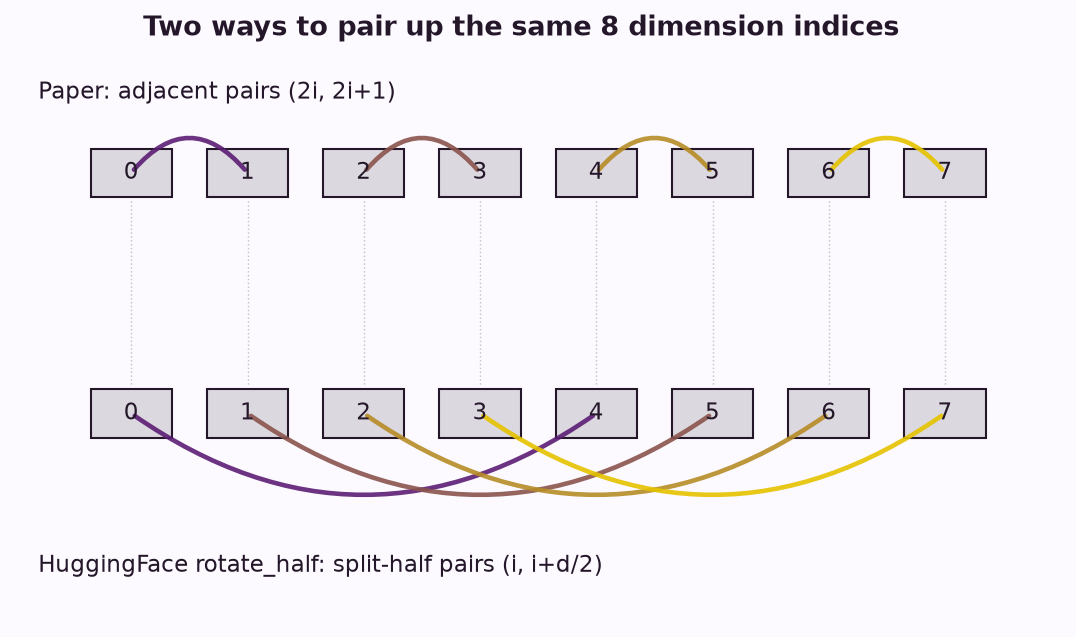
\includegraphics[width=\linewidth]{figures/dim_pairing_diagram.png}
\caption{两种配对方式：相邻配对与前后半配对。同样的旋转，不同的坐标落位。}
\end{figure}

\section{六、错误的位置永远不报错}

RoPE 在 key 进入 KV 缓存之前作用于它。缓存里的 key 是旋转之后的，它被算出来时所在的那个位置参照系，已经烤进了它的数值。切一个张量是在搬运数字，它不会把一次已经发生的旋转倒回去。

设一段长度为 $p + s$ 的缓存被截断到只剩最后 $s$ 项。活下来的 key 仍然带着来自绝对位置 $[p,\ p+s)$ 的旋转。若下一个 query 的位置改从截断后的缓存长度去取，它落在 $s$，而 key 还在 $p + s$ 附近：

\[
m - n \in (-p,\ s - p].
\]

一旦 $p$ 超过 $s$，每一个相对距离都是负的。query 被当作 key 在它前面那样去旋转，这是因果训练从不产生的排布。

现在回到第二节的 $\|Rv\| = \|v\|$。什么都没坏：没有异常，没有 NaN，没有形状不匹配，没有告警。向量还是它一直以来的长度。动的只有方向，而方向恰好是点积所读的东西。错误落在了决定注意力的那个量上，落在表示里唯一没有任何不变量守着的那一维。

\begin{quote}
一个大声失败的系统会告诉你它在哪里失败。这一个不会。这里的正确性，不能从没有报错推出来。
\end{quote}

\section{七、衰减是免费送的}

把 $q$ 和 $k$ 的分量成对分组，把旋转后的内积写成一列复数项之和。对这个和做一次 Abel 变换，可以把它界住：

\[
\left|\sum_{i=0}^{d/2-1} h_i\, e^{i(m-n)\theta_i}\right|
\le \max_i |h_{i+1} - h_i| \sum_{j=0}^{d/2-1} |S_j|,
\qquad S_j = \sum_{i=0}^{j-1} e^{i(m-n)\theta_i}.
\]

真正衰减的量，是 $|S_j|$ 对 $j$ 取的平均。它只依赖相对距离和频谱，不依赖任何特定的 $q$ 与 $k$。趋势是向下的，但不是单调的：界是一列振荡项之和，个别距离会高过它的邻居，而包络仍在下落。所以读单独一对距离在这里什么也证明不了，成立的是它在一段范围上的形状。

这和第四节合了拢。频谱是为了避免混叠才选的，衰减随它一起到来，没人点单。一个设计决定，两个有用的后果，这是构造并非任意的一个合理信号。

\begin{figure}
\centering
\includegraphics[width=\linewidth]{figures/long_term_decay_animation.gif}
\caption{上界随相对距离的整体走势：向下，但沿途起伏。看一段，不看一点。}
\end{figure}

\section{八、边界}

上面的一切，讲的都是作为数学对象的这个编码。没有一句在讲一个训练好的模型会如何响应。

这条界很容易丢，值得攥住。旋转不知道一个句子是什么。像“误差在短序列上更糟”这样的话，是关于学到的权重和训练分布的断言，拿随机向量怎么测都立不起来，它需要对着具体那个模型去量。

这份推导确实立住的是：不变性成立，范数存活，两种约定在置换下一致、不置换则相左，一个与缓存旋转不自洽的位置会挪动注意力的输出。这些是编码的性质，无论哪个模型拿它去做什么，它们都成立。

对应的代码仓库在 \href{https://github.com/yyfenghuang/RoPE-first-principle}{github.com/yyfenghuang/RoPE-first-principle}，每一条断言都配着一段能跑的代码。原始方法出自 Su 等人的 RoFormer\footnote{Su et al., \emph{RoFormer: Enhanced Transformer with Rotary Position Embedding}, \href{https://arxiv.org/abs/2104.09864}{arXiv:2104.09864}.}。

\end{document}
